\section{Mortality model explanation with SHAP}
The mortality explanation uses the frozen T06 CatBoost base estimator and development predictors only. Native CatBoost Independent TreeSHAP values were calculated on the 1,360 development rows, with a 64-row development reference sample selected using seed 42. The Platt calibrator and decision threshold were not applied to the attribution values; SHAP explains the model's raw score \cite{lundberg2020,prokhorenkova2018}. Figure~\ref{fig:shap} is the summary plot, where features are ordered by mean absolute contribution. The largest mean absolute attributions were AGE (0.2935), ZSN\_A (0.2911), ant\_im (0.2873), TIME\_B\_S (0.2699), and STENOK\_AN (0.2131). The source dictionary describes them as age, chronic heart failure in the anamnesis, anterior MI ECG pattern, time from attack onset to hospital, and prior exertional angina.

These ranks describe contribution magnitude in this fitted model, not causal effects or a uniform direction of effect. The monochrome plot does not encode feature values. The guide's optional local explanations for two example patients are not supplied in this draft.
\begin{figure}[H]\centering
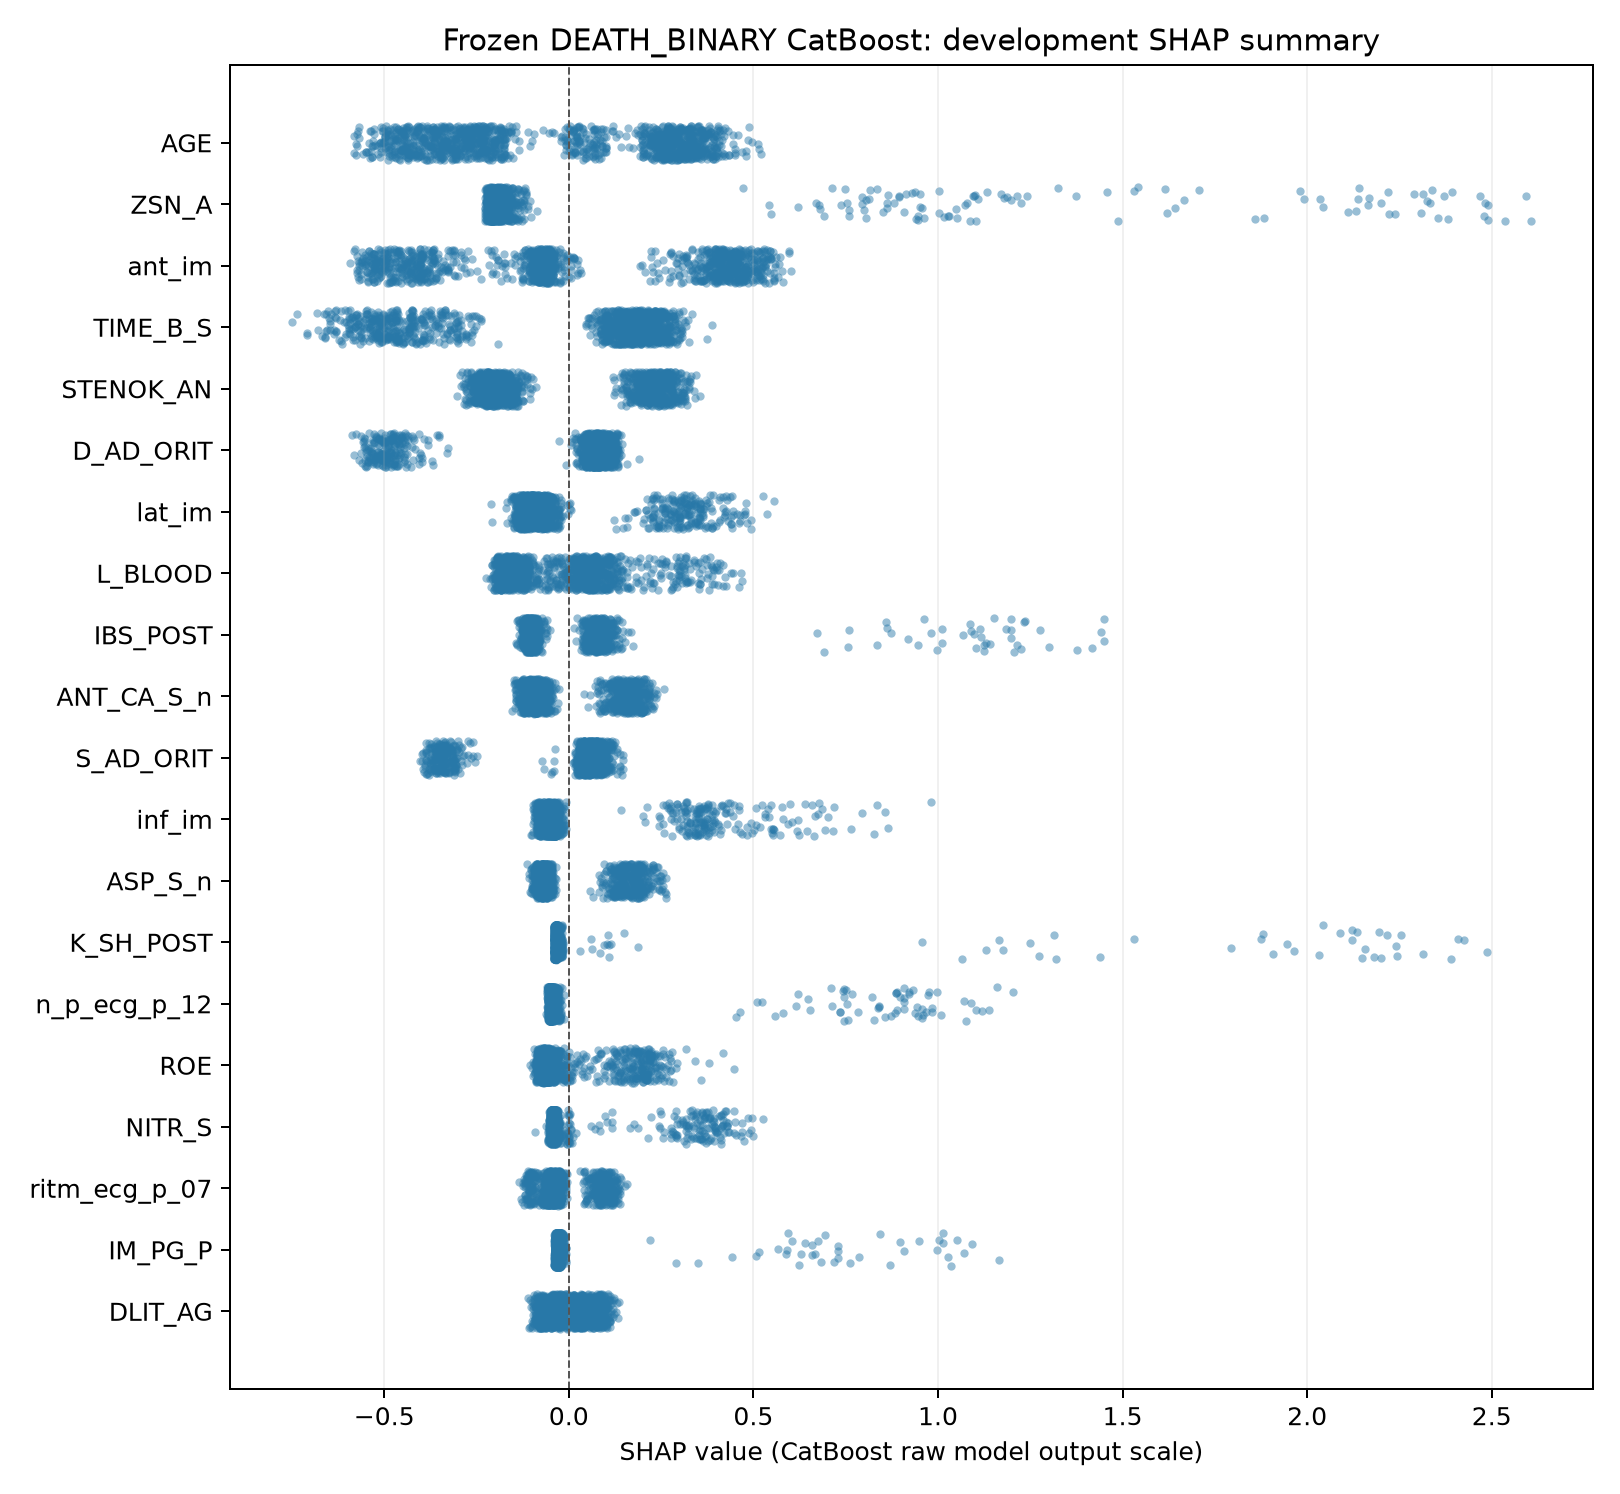
\includegraphics[width=.85\linewidth]{mortality_shap_summary.png}
\caption{Development-only SHAP summary for frozen mortality CatBoost. Source: \texttt{stage13\_t09\_mortality\_shap\_outputs/mortality\_shap\_summary.png}.}\label{fig:shap}
\end{figure}
